\section{Experimental Design}

\subsection{Sample Preparation}

The sample used in this experiment is the same one which was used in the Phys 437A project. For the sake of brevity this section will serve only as a review of the sample preparation procedure. 

A Copper single crystal with dimensions 10mm $\times$ 10mm $\times$ 1mm was chosen for the experiment, with the $[111]$ direction being normal to the sample's surface. The sample was 
cleaned chemically first using a dilute acid wash, followed by cleaning with a series of organic solvents. The sample was transferred to the prep chamber of our spectrometer and 
cycled through Argon ion etching and annealing at $400^\circ$C\cite{robinson2012argon} until the resulting low energy electron diffraction pattern was sharp and well ordered. 

After completing the Phys 437A project the sample was left in the spectrometer's IPES (main) chamber under high vacuum conditions, being exposed to pressures no higher than $9\times10^{-10}$ torr.


\subsection{The IPES Chamber}

The experiment was conducted within the IPES vacuum chamber portion of our spectrometer. Within the chamber is a motorized sample holder with the ability to translate along $x$, $y$ and $z$ 
directions, with $z$ denoting the central axis of the chamber. A design diagram is presented in figure \ref{fig:holder}. The holder is also capable of rotation about the $z$ axis with the rotation angle denoted $\theta$. A sample can be
secured to this holder which allows for it to be positioned in the output of the electron gun. The current from the electron gun can be measured as the total current reaching the 
sample, or as the current at a certain location in space using a Faraday cup mounted above the sample. A Faraday cup is a conductive cup with a pinhole sized opening, meaning only the portion 
of the beam which intersects the pinhole will contribute to the current measurement. Keithley Instruments 6485 and 6487 picoammeters are used to record these currents, which are connected to 
the chamber using coaxial cable vacuum feedthroughs. The sample and Faraday cup share a common ground and can be biased to positive or negative potentials using the Keithley 6487's
voltage supply. This setup allows for high accuracy measurements of both the beam intensity and shape, and determining the sample's contact potential.

\begin{figure}[h!]
    \centering
    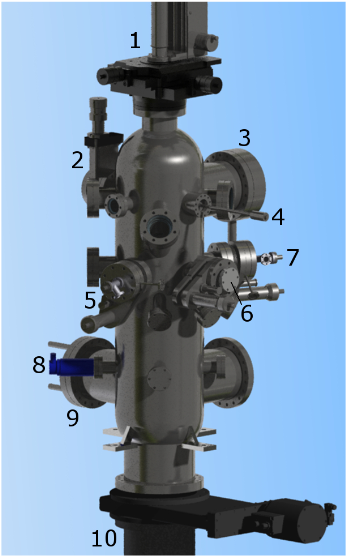
\includegraphics[scale=0.35]{../Assets/IPES.png}
    \hfil
    \includegraphics[scale=0.35]{../Assets/sample holder.png}
    \caption{Left: Diagram of IPES chamber showing the manipulator stage (1), electron gun (6), photodetectors (5, 7), and cryopump (10). 
    Right: Sample holder diagram, showing relative position of mounted sample (orange) and faraday cup. Coordinate axes indicate translational directions
    and direction of increasing $\theta$ can be seen\cite{mcmahon_2012}.}
    \label{fig:holder}
\end{figure}

\clearpage
The electron gun in our system is a commercially available design produced by Staib Instruments. The specific model, NEK-150, is reported to achieve a current of 5$\mu$A and a spot size of 1mm at electron 
energies below 10eV\cite{staib}. 

These devices are all interfaced to a computed through a labVIEW control program. It is capable of recording the current readings from the ammeters, setting the bias voltage applied 
to the sample and faraday cup, and controlling the electron gun. Custom scanning programs can be written to vary instrument parameters and record resulting measurements. 

\subsection{Procedure}

The desired operating parameters for the gun are fist set using the labVIEW control program. For contact potential and energy resolution determination, the sample is maneuvered in front 
of the electron gun at a set working distance. The Keithley 6487 is used to bias the sample over a set range of voltage values with a given voltage increment. At each step of increasing 
the bias the sample current is recorded, also done using the 6487 picoammeter. The Faraday cup can be used instead of the sample itself if the goal is to observe the energy distribution 
of the beam at specific locations. 

Measuring the width of the beam is done using the Faraday cup. The cup is aligned with the beam, and then translated along a direction perpendicular to the beam's axis. For most 
runs in this experiment the direction chosen was the $x$ direction, with the beam aligned along the $y$ direction of figure \ref{fig:holder}. Once the Faraday cup is translated completely 
out of the beam, a scan is started to increment its position such that it traverses across the entire beam. At each position the picoammeter records the current of the beam, as well 
as the position readout from the motor's rotary encoder. It will be seen in the results that the absolute position values across different measurements 
can vary significantly. The reason for this is a reset of the motor position, with zero representing the position of the motor on start up. This has no effect on the results presented since only 
relative distances are important for any calculations, and any qualitative behaviour can be understood by using the coordinate axes of the spectrometer.

The above procedure can be further expanded by adding an additional scanning direction. Allowing the Faraday cup to scan in the $z$ direction as well as the $x$ direction will create a 
raster scan. This is particularly useful to gauge the symmetry of the beam, since a while behaved beam should be rotationally symmetric about its axis. If instead the Faraday cup is 
moved in a combination of $y$ and $x$ directions the beam width at different working distances can be found. This allows for the beam's divergence angle to be computed, which can be 
used to determine the broadening in the beam's momentum distribution. 

Finally, KRIPES measurements are taken by setting an incidence angle, $\theta$, using the rotational motor. The photodetectors are then filled with acetone to the appropriate pressure, and 
the corresponding high voltage is applied to the anode wire. The photodetector configurations were determined previously through experiment in Phys 437A. 
The electron gun sweeps through a set range of $E_i$ values and records the number of detections which come from the photodetectors. 
The incident angle can be varied and the scan repeated to show how the unoccupied states change with momentum. 

The process of characterizing the electron gun involved examining a wide range of operating parameters and testing the beam's performance using the first two experiments. Once a 
good configuration was found it was further studied using raster scans and longitudinal scans. The fully characterized beam was finally used for a series of k 
resolved inverse photoemission measurements, which could then be compared to results reported in literature. 